\chapter{Theoretical and experimental background} % (fold)
\label{cha:theoretical_background}
%%%%%%%%%%%%%%%%%%%%%%%%%%%%%%%%%%%%%%%%%%%%%%%%%%%%%%%%%%%%%%%%%%%%%%%%%%%%%%%%%%%%%%%%%%%%%%%%%%%%%%%%%%%%%%%%%%
%%%%%%%%%%%%%%%%%%%%%%%%%%%%%%%%%%%%%%%%%%%%%%%%%%%%%%%%%%%%%%%%%%%%%%%%%%%%%%%%%%%%%%%%%%%%%%%%%%%%%%%%%%%%%%%%%%
%%%%%%%%%%%%%%%%%%%%%%%%%%%%%%%%%%%%%%%%%%%%%%%%%%%%%%%%%%%%%%%%%%%%%%%%%%%%%%%%%%%%%%%%%%%%%%%%%%%%%%%%%%%%%%%%%%
%%%%%%%%%%%%%%%%%%%%%%%%%%%%%%%%%%%%%%%%%%%%%%%%%%%%%%%%%%%%%%%%%%%%%%%%%%%%%%%%%%%%%%%%%%%%%%%%%%%%%%%%%%%%%%%%%%
%%%%%%%%%%%%%%%%%%%%%%%%%%%%%%%%%%%%%%%%%%%%%%%%%%%%%%%%%%%%%%%%%%%%%%%%%%%%%%%%%%%%%%%%%%%%%%%%%%%%%%%%%%%%%%%%%%
\section{Attosecond dynamics} % (fold)
\label{sec:attosecond_dynamics}

Understanding and imaging motion on fast time scales has been of interest for centuries. In 1877, Eadweard Muybridge invented high speed photography to find out if all of a horse's feet leave the ground at a full gallop. Since then, high speed photography has reached time scales of $\sim10^{-5}$s, a long ways off of the attosecond ($10^{-18}$s) time scale of electron motion. On attosecond time scales, only electrons in atoms and molecules display significant motion (see Fig.~\ref{fig:time_scales}) rendering electronic or mechanical shutters, from traditional photography, useless. Additionally, the electrons being imaged are quantum objects further complicating the imaging process. Before we go into the methods used for imaging electron motion, lets dive into what we mean when we say a quantum object is moving. 

For a time independent system, such at an atom or molecule in vacuum, there exists a set of stationary states that are eigenfunctions of the system's Hamiltonian (for details see Sec.~\ref{sec:TDSE}). In the case of an atom or molecule, these stationary states are the bound or continuum states which we will call $\ket{\psi_j(\mathbf{r})}$. These states depend on space, and evolve in time like $e^{iE_j t}$ where $E_j$ is the energy of the $j$th stationary state, $i=\sqrt{-1}$ is the imaginary number, and $t$ is time. This shows that only the phase of the state is changing in time. As the global phase of a wavefunction is not observable, an electron occupying a single stationary state displays no motion. 

For attosecond motion to occur, either the system's Hamiltonian must become time dependent, such as introducing a laser pulse, and/or multiple stationary states must be populated forming a superposition. The former is often required to image the motion of electrons, but the latter is simpler to understand. We will therefore start with the motion produced by an electron in a superposition of more than one stationary state. In principle, one or more of the states could be a continuum states, but for simplicity we restrict ourselves to bound states only in the following discussion. The resulting electronic wavefuction can be written as
\begin{equation}
\label{eq:atto_dynamics}
    \ket{\Psi(\mathbf{r},t)} = \sum_{j=0}^{N-1} a_j e^{i(\phi_j +E_jt)}\ket{\psi_j(\mathbf{r})}
\end{equation}
where $a_i$ is a non negative real number, $\phi_i$ is a phase, and the superposition contains $N$ total states each labeled by the subscript $j$. The global phase can be accounted for by removing the time dependent phase of the ground states ($j=0$). The resulting relative phase of the excited states ($j>0$) changes in time like $(E_j-E_0)t$ resulting in dynamics if $E_j\ne E_0$. For a two state system, the dynamics will be periodic with a period of $T=2\pi/|E_1- E_0|$. Fig.~\ref{fig:he_dynamics} shows the dynamics of the wavefunction for a helium atom in a $1s-2p_+$ superposition as it rotates with a period of approximately 200 attosecond. 
\begin{figure}[!ht]
\centering
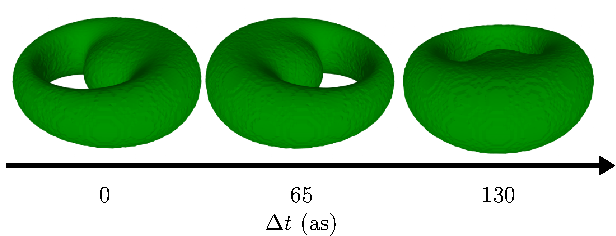
\includegraphics[width=\columnwidth]{figs/background/dynamics.pdf}
\caption{\label{fig:he_dynamics} An isosurface of the wavefunction of a helium atom in a $1s-2p_+$ superposition ($|r\Psi|$) undergoing attosecond motion. (figure from \cite{venzke2021_wave})
}
\end{figure}
Adding additional states to the superposition allows for arbitrarily complicated field free dynamics to occur. In order to ``image'' the wavepacket, all of the values for $a_j$ and $\phi_j$ must be obtained at some time $t_0$ with the restrictions that $a_0 = \sqrt{1-\sum_{j=1}^{N-1} a_j^2}$ and $\phi_0=0$ to enforce normalization and removing the global phase respectively. Then using eq.~\ref{eq:atto_dynamics}, the time dependence of the system is known. A method for imaging simple superpositions is presented in Sec.~\ref{sec:wavefunction_reconstruction}.

When the system's Hamiltonian becomes time dependent, however, the above approach does not capture the dynamics completely. If the time dependent operator is weak relative to the time independent operators, the dynamics maybe captured by allowing $a_j$ and $\phi_j$ to become time dependent quantities. When the time dependent operator becomes comparable or larger than the independent operators, the stationary states, $\ket{\psi_j(\mathbf{r})}$, may no longer be a good basis to describe the system. Imaging the dynamics of such a system would requires techniques beyond the scope of this thesis.
% section attosecond_dynamics (end)

%%%%%%%%%%%%%%%%%%%%%%%%%%%%%%%%%%%%%%%%%%%%%%%%%%%%%%%%%%%%%%%%%%%%%%%%%%%%%%%%%%%%%%%%%%%%%%%%%%%%%%%%%%%%%%%%%%
%%%%%%%%%%%%%%%%%%%%%%%%%%%%%%%%%%%%%%%%%%%%%%%%%%%%%%%%%%%%%%%%%%%%%%%%%%%%%%%%%%%%%%%%%%%%%%%%%%%%%%%%%%%%%%%%%%
%%%%%%%%%%%%%%%%%%%%%%%%%%%%%%%%%%%%%%%%%%%%%%%%%%%%%%%%%%%%%%%%%%%%%%%%%%%%%%%%%%%%%%%%%%%%%%%%%%%%%%%%%%%%%%%%%%
%%%%%%%%%%%%%%%%%%%%%%%%%%%%%%%%%%%%%%%%%%%%%%%%%%%%%%%%%%%%%%%%%%%%%%%%%%%%%%%%%%%%%%%%%%%%%%%%%%%%%%%%%%%%%%%%%%
%%%%%%%%%%%%%%%%%%%%%%%%%%%%%%%%%%%%%%%%%%%%%%%%%%%%%%%%%%%%%%%%%%%%%%%%%%%%%%%%%%%%%%%%%%%%%%%%%%%%%%%%%%%%%%%%%%
\section{Pump-probe spectroscopy} % (fold)
\label{sec:pump_probe_spectroscopy}
Pump-probe spectroscopy is a powerful tool for imaging ultrafast processes. The general concept is quite simple. Two isolated ultrafast pulses are produced. The first pulse, known as the probe pulse, prepares the system by starting some dynamic process. Some time after the end of the first pulse, the second (probe) pulse images the target. By delaying the probe pulse with respect to pump pulse, the impact of the dynamics on a given observable can be observed experimentally. This gives a glimpse at how the system evolves overtime. Although conceptually easy to understand, attosecond pump-probe spectroscopy is an extremely difficult experiment to preform. 

In many cases, it is needed to have both angle and/or energy spectra of the ionized electrons. The development of experimental techniques, such as velocity map imaging (VMI) \cite{kornilov2010,rouzee2011} or cold target recoil ion momentum spectroscopy (COLTRIMS) \cite{ullrich2003}, the detection of angle-resolved emission of the photoelectron following few-photon ionization of atomic and molecular targets has become possible \cite{ma2013}. 
Additionally, one requires the ability to produce well controlled isolated ultrafast laser pulses. In the recent past, it has become possible to generate isolated attosecond pulses \cite{frank2010}. This has opened the door for the application of pump-probe spectroscope to attosecond physics. In 2001, the first experimental observation of attosecond electron dynamics was made with a pump-probe setup including an few cycle visible light pulse and an attosecond soft-X-ray pulse \cite{hentschel2001}. The bandwidth of attosecond laser pulses allow for both bound and continuum states to be studied \cite{mauritsson2010} and, more recently, charge dynamics in Tryptophan on the sub 4fs time scale have been observed opening the door for attosecond pump-probe spectroscopy to be used on complex molecules \cite{larasstiaso2018}. As experimental techniques evolve, the application of attosecond pump-probe experiments will continue to expand. In this thesis, we look at how pump-probe spectroscopy can be used to understand the ionization of electrons in superposition states in Sec.~\ref{sec:generalized_asymmetry_parameters} and reconstruct attosecond electron motion in Sec.~\ref{sec:wavefunction_reconstruction}.
% section pump_prop_spectroscopy (end)

%%%%%%%%%%%%%%%%%%%%%%%%%%%%%%%%%%%%%%%%%%%%%%%%%%%%%%%%%%%%%%%%%%%%%%%%%%%%%%%%%%%%%%%%%%%%%%%%%%%%%%%%%%%%%%%%%%
%%%%%%%%%%%%%%%%%%%%%%%%%%%%%%%%%%%%%%%%%%%%%%%%%%%%%%%%%%%%%%%%%%%%%%%%%%%%%%%%%%%%%%%%%%%%%%%%%%%%%%%%%%%%%%%%%%
%%%%%%%%%%%%%%%%%%%%%%%%%%%%%%%%%%%%%%%%%%%%%%%%%%%%%%%%%%%%%%%%%%%%%%%%%%%%%%%%%%%%%%%%%%%%%%%%%%%%%%%%%%%%%%%%%%
%%%%%%%%%%%%%%%%%%%%%%%%%%%%%%%%%%%%%%%%%%%%%%%%%%%%%%%%%%%%%%%%%%%%%%%%%%%%%%%%%%%%%%%%%%%%%%%%%%%%%%%%%%%%%%%%%%
%%%%%%%%%%%%%%%%%%%%%%%%%%%%%%%%%%%%%%%%%%%%%%%%%%%%%%%%%%%%%%%%%%%%%%%%%%%%%%%%%%%%%%%%%%%%%%%%%%%%%%%%%%%%%%%%%%
\section{Few photon ionization} % (fold)
\label{sec:few_photon_ionization}
Multiphoton ionization was proposed by Maria G\"oppert-Mayer in 1931 \cite{goppertmayer1931}. Thirty years later, two photon ionization was demonstrated experimentally shortly after the advent of the laser \cite{kaiser1961}. As we approach a century since the proposal of multiphoton ionization, research in this area is still alive and well. With recent advances in HHG and FEL laser pulse sources in the extreme-ultraviolet (EUV) colors, studies involving few photon ionization in the perturbative intensity regime have been of both experimental and theoretical interest \cite{nikolopoulos2001,vanderhart2005,shakeshaft2007,pi2010,florescu2011,sato2011,haber2011,florescu2012,ishikawa2012,ishikawa2013,ma2013,rey2014,grum-grzhimailo2015,douguet2016,hofbrucker2017,hofbrucker2018,boll2019,wang2019}. Using tools like VIM and COLTRIMS allows for both the direction and momentum of the ionized electrons to be detected. At a given electron energy, the probability distribution of an electron being ionized in a specific direction is known as a photoelectron angular distributions (PAD). 

PADs contain information containing to both the phase and amplitude of the various partial waves produced during the ionization process. These signals have been used to study thee competition between resonant and non-resonant two-photon ionization pathways \cite{ishikawa2012,ishikawa2013,ma2013} and for one- and two-photon ionization channels \cite{grum-grzhimailo2015,douguet2016,boll2019}.
These tools are also used to investigate the impacts of many physical effects, such as a significant circular dichroism via the asymmetry in the forward-backward electron emission from bromocamphor molecules induced by circularly polarized light has been identified  \cite{bowering2001}. Observation of the breakdown of the symmetry in the photoelectron emission of argon has been shown in the region of the Cooper minimum \cite{ilchen2018}, molecular vibrations and chirality \cite{garcia2013} and applications range from studies of coherent control \cite{prince2016} to the characterization of ultrashort laser pulses \cite{chelkowski2002}.

The contents of Chap.~\ref{cha:imaging_wave_packets_with_photoelectrons} dive into the impacts of few photon ionization using ultrashort pulses (Sec.~\ref{sec:short_pulse_effect}), proposing new asymmetry parameters for understanding few photon ionization of electrons in superpositions  (Sec.~\ref{sec:generalized_asymmetry_parameters}) and how few photon ionization can be used to reconstruct attosecond electron motion (Sec.~\ref{sec:wavefunction_reconstruction}).
% section few_photon_ionization (end)

%%%%%%%%%%%%%%%%%%%%%%%%%%%%%%%%%%%%%%%%%%%%%%%%%%%%%%%%%%%%%%%%%%%%%%%%%%%%%%%%%%%%%%%%%%%%%%%%%%%%%%%%%%%%%%%%%%
%%%%%%%%%%%%%%%%%%%%%%%%%%%%%%%%%%%%%%%%%%%%%%%%%%%%%%%%%%%%%%%%%%%%%%%%%%%%%%%%%%%%%%%%%%%%%%%%%%%%%%%%%%%%%%%%%%
%%%%%%%%%%%%%%%%%%%%%%%%%%%%%%%%%%%%%%%%%%%%%%%%%%%%%%%%%%%%%%%%%%%%%%%%%%%%%%%%%%%%%%%%%%%%%%%%%%%%%%%%%%%%%%%%%%
%%%%%%%%%%%%%%%%%%%%%%%%%%%%%%%%%%%%%%%%%%%%%%%%%%%%%%%%%%%%%%%%%%%%%%%%%%%%%%%%%%%%%%%%%%%%%%%%%%%%%%%%%%%%%%%%%%
%%%%%%%%%%%%%%%%%%%%%%%%%%%%%%%%%%%%%%%%%%%%%%%%%%%%%%%%%%%%%%%%%%%%%%%%%%%%%%%%%%%%%%%%%%%%%%%%%%%%%%%%%%%%%%%%%%
\section{Rydberg state excitations induce by strong fields} % (fold)
\label{sec:rydberg_state_excitations_induce_by_strong_fields}
% Fundamental processes in strong-field atomic physics are above-threshold ionization (ATI), high harmonic generation (HHG) and non-sequential double ionization. These highly nonlinear processes are induced by the absorption of multiple photons from the laser field, which in the limit of a large photon number can also be described as a tunneling process. 
Excitation of the atom is known to play an important role in each of the processes. It has been initially observed via resonant enhancement in the population of excited states \cite{deboer1992,jones1992} and structures in the energy spectrum \cite{freeman1987,perry1989,agostini1989} and in energy-resolved angular distributions \cite{rottke1994} of photoelectrons. These resonance effects have been explained by multiphoton absorption through Rydberg states, which are AC-Stark shifted in the presence of a laser field. More recently, significant excitation of atoms has also been observed in the tunneling regime and described by the frustrated tunneling ionization model. 

For linearly polarized lasers, the latter observation has renewed the general interest in the mechanisms leading to the population of excited (Rydberg) states during the interaction of an atom with an intense laser pulse (most recently, e.g., in Refs. \cite{chini2014,li2014,li2014b,zimmermann2015,shao2015,camp2015,li2015,fechner2015,bredtmann2016,fushitani2016,lv2016,serebryannikov2016,hart2016,li2016,xiong2016,beaulieu2016,larimian2016,zimmermann2017,bengtsson2017,gao2017,ivanov2017,ilchen2017,mancuso2017,xiong2017,piraux2017}). The important role of Rydberg states in various strong-field ionization processes and harmonic generation has been discussed. For example, resonant enhancement of below-threshold harmonics \cite{toma1999,chini2014,camp2015}, emission from excited states via free induction decay \cite{camp2015,beaulieu2016}, high harmonic emission through ionization from excited states and recombination to the ground state \cite{bian2010,beaulieu2016} have been predicted and observed.

Recent theoretical studies of the excitation mechanism in linearly polarized strong fields mainly consider the distribution of the population as a function of the principal quantum number of the excited states \cite{li2014,li2014b,zimmermann2017,xiong2017,piraux2017}. It was shown that the modulation of the excitation probability is related to the channel closing effect \cite{krajewska2012,li2014,li2014b,piraux2017}. The latter phenomenon occurs at threshold intensities at which the absorption of one more photon is needed to ionize the atom due to the shift of the ionization threshold by the ponderomotive energy. The interpretation that an increase in excitation can be understood as result of the shift of the first ATI peak below the ionization threshold \cite{li2014,li2014b} is in agreement with the explanation of earlier experimental results (e.g., \cite{freeman1987,jones1992,rottke1994}) via the resonance enhanced population of AC-Stark shifted excited states. 

Theoretical analysis of the angular momentum distribution in the populated Rydberg states by linearly polarized fields is less advanced. Predictions of Floquet theory for a monochromatic laser field \cite{krajewska2012} and results of numerical calculations for laser pulses with a trapezoidal envelope \cite{piraux2017} yield that the angular momentum of the excited Rydberg states has the same parity as $N_p-1$, where $N_p$ is the minimum number of photons needed to ionize the atom. Furthermore, the angular quantum number of the states with the largest population in numerical calculations \cite{li2014,li2014b,piraux2017} agrees well with semiclassical estimations \cite{arbo2008}, initially performed for low-energy angular resolved photoelectron distributions.

Besides interactions with linear polarized laser pulses, recently studies on the interaction of atoms and molecules with intense fields generated by the superposition of two circularly polarized laser pulses have seen an upsurge in activity in strong-field experiment and theory. For the most part, the renewed interest results from the capability to control the polarization of emitted light in high-order harmonic generation with such pulses. The physical principle has been proposed and applied first two decades ago 
\cite{eichmann1995,long1995}. 
More recently, efficient phase matching of circularly polarized high-order harmonic beams in the EUV and soft X-ray regime using bichromatic beams with counter-rotating circular polarization has been demonstrated \cite{fleischer2014,pisanty2014,kfir2015,fan2015,hickstein2015}. Since then, much experimental and theoretical work on high-harmonic generation \cite{milosevic2015a,medisauskas2015,milosevic2015b,chen2016,baykusheva2016,hernandez2016,liu2016,mauger2016,bandrauk2016,reich2016b,odzak2016,dorney2017,fleischer2017,zhavoronkov2017,pisanty2017,baykusheva2017,lerner2017,ayuso2018,dixit2018,barreau2018,huang2018,jimenez2018,heslar2018,paufler2018,li2019}, 
ionization and photoelectron momentum distributions
\cite{ngoko2015,yuan2016,milosevic2016c,mancuso2016,milosevic2016b,mancuso2017,pengel2017,busuladzic2017,hoang2017,lin2017,abusamha2018,busuladzic2018,eckart2018,li2018,han2018,eckart2018b,liu2018,eicke2019,ge2019,kerbstadt2019,abusamha2019}, double ionization 
\cite{mancuso2016b,eckart2016,ben2017,ngoko2017,yu2018,huang2018b,ma2019}
and other strong-field processes \cite{yuan2015,buica2018,guo2019} driven by bichromatic circularly polarized laser pulses has been performed. One interesting aspect in these kind of strong-field interactions is the control of ionization via the helicity of the applied bichromatic pulses \cite{milosevic2016c,mancuso2016,liu2018}. Such studies complement related work on the dependence of the ionization rate by one-color circularly pulse on the relative helicity between the pulse and the electron in the atomic orbital
\cite{barth2011,kazansky2012,herath2012,barth2013,bauer2014,barth2014,ooi2014,hartung2016,douguet2016,watzel2016,wang2017,zhang2017,eckart2018c,liu2018b,trabert2018}.

For the interaction with bichromatic circularly polarized laser pulses resonant excitation also plays an important role. It has been observed that the probability to ionize an atom is significantly enhanced if the two fields are counter-rotating as compared to co-rotating fields \cite{mancuso2016}. The experimental observations were interpreted as due to the increased density of excited states accessible for resonant enhanced multiphoton ionization in the case counter-rotating fields. Results of numerical solutions of the time-dependent Schr\"odinger equation in Ref.\ \cite{mancuso2016} did confirm a close relation between the ratios of total excitation and ionization probabilities for counter-rotating and co-rotating circularly polarized laser pulses. However, the results for excitation of the atom were not further resolved by distributions over the quantum numbers (principal, angular momentum, magnetic). Such analysis potentially can shed further light on the role of excited states in the pathways to ionization since excitation in a resonant multiphoton process should rely on the spin-angular momentum selection rules for the absorption of circularly polarized photons ($\Delta l = \pm 1$ and $\Delta m = \pm 1$).
% section rydberg_state_excitations_induce_by_strong_fields (end)

%%%%%%%%%%%%%%%%%%%%%%%%%%%%%%%%%%%%%%%%%%%%%%%%%%%%%%%%%%%%%%%%%%%%%%%%%%%%%%%%%%%%%%%%%%%%%%%%%%%%%%%%%%%%%%%%%%
%%%%%%%%%%%%%%%%%%%%%%%%%%%%%%%%%%%%%%%%%%%%%%%%%%%%%%%%%%%%%%%%%%%%%%%%%%%%%%%%%%%%%%%%%%%%%%%%%%%%%%%%%%%%%%%%%%
%%%%%%%%%%%%%%%%%%%%%%%%%%%%%%%%%%%%%%%%%%%%%%%%%%%%%%%%%%%%%%%%%%%%%%%%%%%%%%%%%%%%%%%%%%%%%%%%%%%%%%%%%%%%%%%%%%
%%%%%%%%%%%%%%%%%%%%%%%%%%%%%%%%%%%%%%%%%%%%%%%%%%%%%%%%%%%%%%%%%%%%%%%%%%%%%%%%%%%%%%%%%%%%%%%%%%%%%%%%%%%%%%%%%%
%%%%%%%%%%%%%%%%%%%%%%%%%%%%%%%%%%%%%%%%%%%%%%%%%%%%%%%%%%%%%%%%%%%%%%%%%%%%%%%%%%%%%%%%%%%%%%%%%%%%%%%%%%%%%%%%%%
\section{Electron correlation} % (fold)
\label{sec:electron_correlation}
\begin{itemize}
    \item Auger decay
    \item autoionizing
    \item NSDI
    \item shake-up/down/off
\end{itemize}

Interferences between resonant and non-resonant pathways \cite{ishikawa2012} or direct and autoionizing channels \cite{cirelli2018} can be identified via anisotropy and asymmetry parameters. Other examples can be found in double photoionization \cite{maulbetsch1992}
% section electron_correlation (end)

% chapter theoretical_background (end)